\chapter{Lagrange Multipliers}

\section{Method of Lagrange Multipliers}

\begin{theorem}
    To find the maximum and minimum values of $f(x, y, z)$ subject to the constraint $g(x, y, z) = k$ [assuming that these extreme values exist and $\nabla g \neq 0$ on the surface $g(x, y, z)=k$]:
    \begin{enumerate}
        \item Find all values of $x, y, z$ and $ \lambda $ such that
            \begin{equation}
                \label{eq: Lagrange Multipliers}
                \nabla f(x, y, z) = \lambda \nabla g(x, y, z)
            \end{equation}
            and
            \begin{equation}
                \label{eq: Lagrange Multipliers}
                \nabla g(x, y, z) = k
            \end{equation}
        \item Evaluate $f$ at all the points $(x, y, z)$ that result from step 1. The largest of these values is the maximum value of $f$; the smallest is the minimum value of $f$.
    \end{enumerate}
\end{theorem}

\begin{flushleft}
    If we write the vector equation $\nabla f = \lambda \nabla g$ in terms of components, then the equations in step 1 become
    \begin{equation}
        \label{eq: Lagrange Multipliers}
        f_x = \lambda g_x \ \ \ f_y=\lambda g_y \ \ \ f_z=\lambda g_z \ \ \ g(x, y, z) = k
    \end{equation}
\end{flushleft}

\begin{flushleft}
    This is a system of four equations in the four unknowns $x, y, z$ and $\lambda$, and we must find all possible solutions (although the explicit values of $\lambda$ are not needed for the conclusion of the method).
\end{flushleft}

\begin{flushleft}
    Given $x=x_0, y=y_0, z=z_0$ is a solution to this system of equations, we have
    
    \begin{enumerate}
        \item if the value of $\lambda$ is 0, then $\nabla f(x_0, y_0, z_0)=0$ and so  $(x_0, y_0, z_0)$ is a critical point of $f$.
        \item if $\lambda$ is not 0, then $\lambda f(x_0, y_0, z_0)$ and $\lambda f(x_0, y_0, z_0)$ are parallel.
        \end{enumerate}
\end{flushleft}

\subsection{Example 1}

Find the extreme values of the function $ f(x, y)=x^2 + 2y^2 $ on the circle $ x^2 + y^2=1 $

\begin{figure}
    \centering
    \subfloat
        \centering
        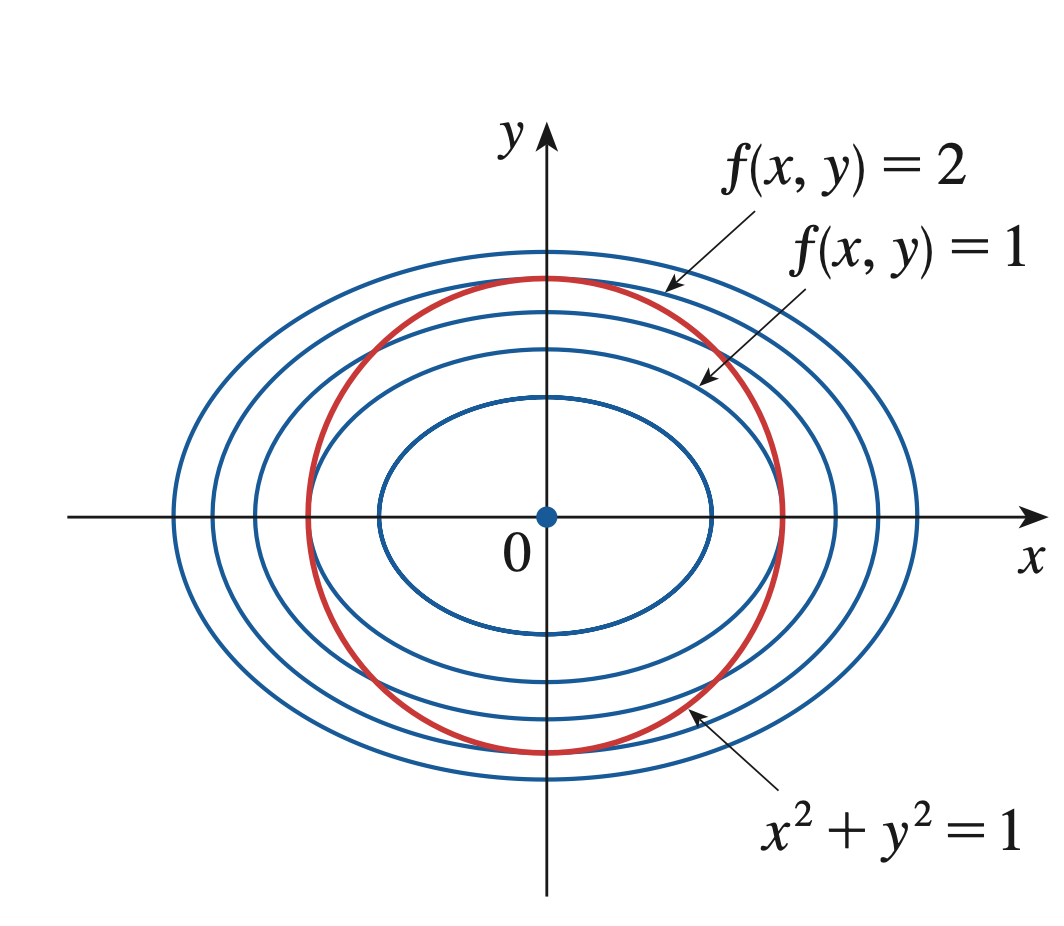
\includegraphics[width=5cm]{chapter003/figures/fig002}
    \qquad
    \subfloat
        \centering
            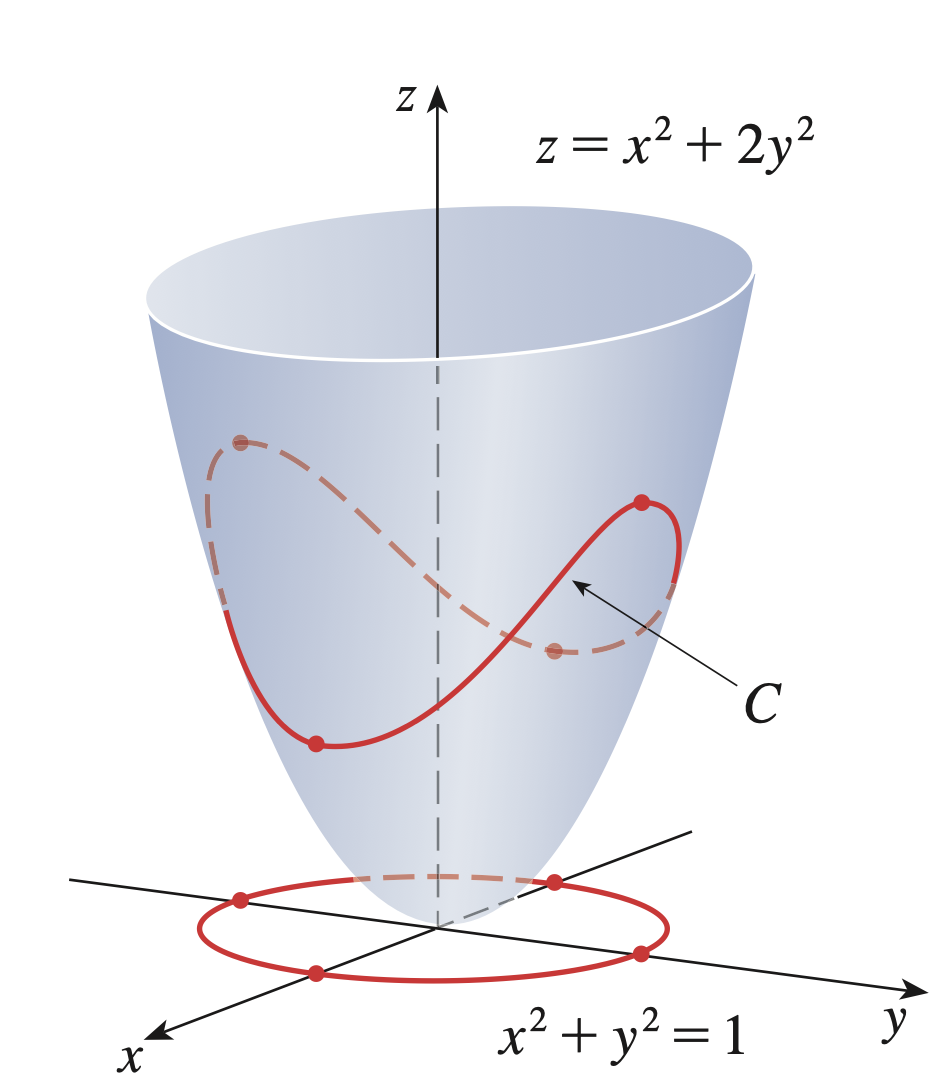
\includegraphics[width=5cm]{chapter003/figures/fig001}
    \label{fig:example}
\end{figure}

\subsubsection{Solution}
We are asked for the extreme values of $f$ subject to the constraint $g(x, y)=x^2 + y^2=1$. Using Lagrange multipliers, we solve the equations $g(x, y)=x^2 + y^2=1$. Using Lagrange multipliers, we solve the equations $\nabla f = \lambda \nabla g$ and $g(x, y)=1$, which can be written as
\begin{equation}
    f_x = \lambda g_x \ \ \ f_y = \lambda g_y \ \ \ g(x, y)=1
\end{equation}
where
\begin{equation}
    f_y = 2x \ \ \ f_y = 4y \ \ \ g_x = 2x \ \ \ g_y = 2y
\end{equation}
then,
\begin{equation}
    2x = \lambda 2x \ \ \ 4y = \lambda 2y \ \ \ x^2 + y^2 = 1
\end{equation}
thus,

\begin{equation}
    2x(1 - \lambda) = 0 \Leftrightarrow
  \left\{
    \begin{aligned}
      & \lambda = 1 \Leftrightarrow y = 0 \Leftrightarrow x= \pm 1\\
      & x = 0 \Leftrightarrow y = \pm 1\ (x^2 + y^2=1)
    \end{aligned}
  \right.
\end{equation}

Therefore, $f$ has possible extreme values at the points $(0, 1), (0, -1)$ and $(1, 0)$ and $(-1, 0)$. Evaluating $f$ at these four points, we find that
\begin{equation}
    f(0, 1) = 2 \ \ \ f(0, -1) = 2 \ \ \ f(1, 0) = 1 \ \ \ f(-1, 0) = 1
\end{equation}
thus, the maximum value of $f$ on the circle $x^2 + y^2=1$ is $f(0, \pm 1)=2$ and the minimum value is $f(\pm 1, 0)=1$

\section{Applications in Machine Learning}
Consider a $D-$dimensional variable \textbf{$x$} with components $x_1, ..., x_D$.

\begin{align}
    x &= \begin{bmatrix}
           x_{1} \\
           x_{2} \\
           \vdots \\
           x_{D}
         \end{bmatrix}
\end{align}

\begin{flushleft}
The constraint equation $g(x)=0$ then represents a $(D-1)$-dimensional surface in x-space. For example, 3-D function $z=x^2+y^2$ and 2-D function $1=x^2+y^2$ are represented in the following figure. In the latter function, $z$ is now a constant.
\end{flushleft}

\begin{figure}
    \centering
    \subfloat
        \centering
        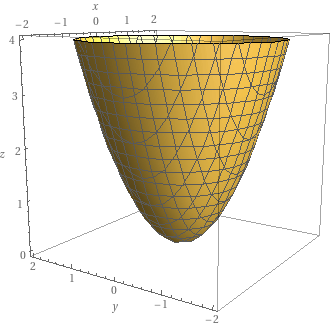
\includegraphics[width=5cm]{chapter003/figures/fig003}
    \qquad
    \subfloat
        \centering
            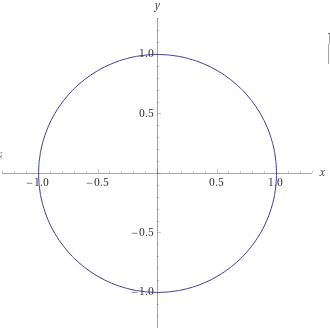
\includegraphics[width=5cm]{chapter003/figures/fig004}
    \label{fig:example}
\end{figure}

According to the equation \ref{eq: Lagrange Multipliers}, we have

\begin{equation}
    \nabla f = \lambda \nabla g \Leftrightarrow \nabla f + \lambda \nabla g = 0
\end{equation}
where $\lambda \neq 0$ is known as a Lagrange multiplier. Note that $\lambda$ can have either sign.

\subsection{Lagrangian function}
\begin{equation}
    \label{eq: Lagrangian function}
    L(x, \lambda) \equiv f(x) + \lambda g(x)
\end{equation}

\begin{flushleft}
Since $\partial L / \partial \lambda = g(x)$, the condition $\partial L / \partial \lambda = 0$ leads to the constraint equation $g(x)=0$.

To find the maximum of a function $f(x)$ subject to the constraint $g(x)=0$, we define the \ref{eq: Lagrangian function} and then find the stationary point of $L(x, \lambda)$ with respect to both $x$ and $\lambda$.
\end{flushleft}

For a $D-$dimensional vector $x$, this gives $D+1$ equations that determine both the stationary point $x*$ and the value $\lambda$. (Why $D+1$ equations? $D$-equations from $x$ and $g(x)=0$)

If we are only interested in $x*$, then we can eliminate $\lambda$ from the stationarity equations without needing to find its value.

As a simple example, suppose we wish to find the stationary point of the function $f(x_1. x_2)=1 - x_1^2 - x_2^2$ subject to the constraint $g(x_1, x_2)=x_1 + x_2 -1 = 0$. The corresponding Lagrangian function is given by 
\begin{equation}
    L(x, \lambda) = 1 - x_1^2 - x_2^2 + \lambda (x_1 + x_2 - 1) = 1 - x_1^2 - x_2^2 + \lambda x_1 + \lambda x_2 - \lambda
\end{equation}

The conditions for this Lagrangian to be stationary with respect to $x_1$, $x_2$ and $\lambda$ give the following coupled equations:

 
\begin{equation}
  \left\{
    \begin{aligned}
      & \frac{\partial L}{\partial x_1} = -2x_1 + \lambda\\
      & \frac{\partial L}{\partial x_2} = -2x_2 + \lambda\\
      & x_1 + x_2 - 1= 0
    \end{aligned}
  \right.
  \Leftrightarrow
  \left\{
    \begin{aligned}
      & x_1 = \frac{1}{2}\\
      & x_2 = \frac{1}{2}\\
      & \lambda = 1
    \end{aligned}
  \right.
\end{equation}

Solution of these equations then gives the stationary point as $(x_1*, x_2*)=(\frac{1}{2}, \frac{1}{2})$ and $\lambda = 1$.






